\chapter{Analyse et conception de la solution SD-WAN }



\section*{Introduction }
Ce chapitre présente l'analyse et la conception de la solution SD-WAN, en mettant l'accent sur le Cisco Viptela SD-WAN. Nous commencerons par une présentation générale de cette technologie avant d'examiner son architecture, ses fonctionnalités et ses composantes principales.

\section{Présentation du Cisco Viptela SD-WAN }
\subsection{Définition du  SDWAN }

Les réseaux SD-WAN (Software-Defined Wide Area Network) sont considérés comme une technologie révolutionnaire pour l'utilisation des services WAN. 

Le SD-WAN introduit le concept de "réseau piloté par les applications",c’est-à-dire le réseau n'est plus statique, mais il s'adapte en temps réel aux exigences des applications et des services utilisés. Sdwan propose une gestion centralisée et flexible et permet d'optimiser l'utilisation des ressources et de garantir une meilleure qualité de service.

Le SD-WAN a un impact majeur sur les services de communication convergente (CC) et les environnements WAN. Il incite à repenser l'utilisation des services réseau et ouvre la voie à de nouvelles possibilités pour la communication du futur.
\subsection{Histoire de Cisco Viptela et son intégration dans l'écosystème Cisco }

Cisco SD-WAN Viptela est issu de l'acquisition de la société Viptela par Cisco en 2017 viptela était reconnue pour sa méthode innovante en matière de SD-WAN en offrant une gestion centralisée et une connectivité sécurisée pour les entreprises distribuées. Son acquisition par Cisco a renforcé l'offre de SD-WAN de l'entreprise et permet une intégration harmonieuse dans l'écosystème Cisco , offrant aussi aux clients une solution SD-WAN complète et performante.
\subsection{Les avantages du cisco viptela SDWAN }

Viptela offre une variété  d'avantages pour les entreprises avec sa capacité à prendre en charge une infrastructure privée en nuage ou sur site, Viptela répond aux besoins de différentes configurations d'infrastructure selon les préférences et les exigences de l'entreprise. 

En offrant une connectivité flexible via des connexions Ethernet, LTE, T1 et DSL, Viptela permet aux entreprises de s'adapter à diverses conditions de connectivité tout en maintenant des performances optimales. Sa prise en charge des topologies WAN complexes avec un haut degré de personnalisation offre une grande souplesse dans la conception et la gestion des réseaux, adaptée aux besoins spécifiques de chaque entreprise.De plus, Viptela fournit une segmentation sécurisée de bout en bout, une gestion des menaces efficace et un contrôle automatisé des chemins, offrant ainsi une tranquillité d'esprit en matière de sécurité et de performances réseau. Son support pour l'intégration de multiples charges de travail virtuelles dans des environnements de cloud privé virtuel (VPC) permet une gestion centralisée et une optimisation des ressources.Bien que le coût par mégabit puisse être légèrement plus élevé en raison de ses fonctionnalités avancées telles que le routage avancé, le chaînage de services et la sécurité cloud, Viptela offre une valeur ajoutée significative en termes de flexibilité, de sécurité et de performances.

En utilisant des équipements tels que les routeurs intégrés ISR 4K ou les vEdge, Viptela garantit une intégration transparente dans l'infrastructure existante, facilitant ainsi la transition vers une solution SD-WAN sophistiquée et évolutive.

\section{Architecture du Cisco Viptela SD-WAN }
\subsection{Architecture logique  }
l'architecture d'un réseau étendu défini par logiciel (SD-WAN) se compose de trois couches superposées de bas en haut comprenant la couche de données, la couche de contrôle et la couche applicative comme montre la figure.
\begin{figure} [H]
	\begin{center}
		\centering
		\hspace*{-0.5cm}
		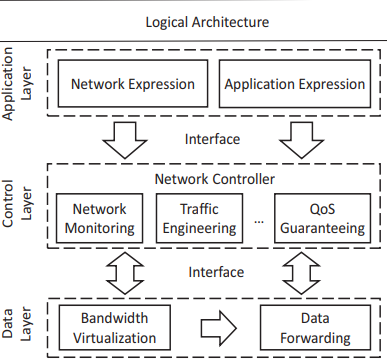
\includegraphics{../image/arch log}
	\end{center}
	\caption{Architecture-logique}
\end{figure} 
\subsubsection{    la couche de données }

Elle assure la virtualisation de bande passante et le transfert de données. la virtualisation de bande passante permet de maximiser l'utilisation des ressources de bande passante en combinant les différents  liens réseau couvrant un même emplacement pour former un pool de ressources partagées, ce qui améliore la performance globale du réseau et permet de répondre de manière plus efficace aux besoins de connectivité des utilisateurs et des applications.

Quant au transfert de données, il est réalisé par un d'éléments de réseau dédié pour le  transfert, principalement des commutateurs, utilisant la capacité de bande passante fournie par la virtualisation de bande passante pour acheminer les paquets de données de manière efficace à travers le réseau . Les deux éléments reçoivent des instructions du contrôleur de réseau situé dans la couche supérieure en utilisant des protocoles d'interface tels que OpenFlow. 
\subsubsection{ la couche de controle}
il existe plusieurs fonctions réseau ,dans la couche de contrôle ,  implémentées et gérées de manière indépendante. La séparation de ces fonctions permet aux opérateurs réseau de développer, de modifier, de déboguer et de supprimer l'une d'entre elles à faible coût sans affecter les autres . ansi les fonctions réseau peuvent être connéctées ,pour offrir une multitude de services et augmenter la flexibilité du réseau étendu défini par logiciel. Prenant par exemple la vue globale fournit par la surveillance du réseau pour l'ingénierie du trafic pour qu’elle puisse calculer une solution d'ordonnancement optimale à exécuter dans le réseau ,aussi La garantie de la qualité de service se charge de satisfaire les exigences des applications pendant la transmission des données. 

\subsubsection{  la couche d’application }
Avec l'émergence croissante d'applications ayant des exigences multiples et parfois contradictoires, il devient essentiel d'adapter les politiques réseau en tenant compte des spécificités de chaque application.
La couche d’application permet aux fournisseurs de réseau et aux développeurs d'applications de participer davantage au contrôle du réseau et de définir leurs exigences spécifiques et de haut niveau pour le réseau à travers l'expression réseau et l'expression d'application. Ces expressions sont capables de traduire ces exigences presque dans un langage naturel en configurations réseau conformes. 
\subsection{Architecture physique }

Dans la couche de données, se trouve un ensemble de commutateurs interconnectés par des liaisons physiques, formant ainsi une infrastructure réseau. Ces commutateurs sont contrôlés par un dispositif central appelé contrôleur réseau. Ce contrôleur peut être un serveur dédié ou un cluster de serveurs, selon la taille et la complexité du réseau. Au-dessus du contrôleur réseau, résident les applications spécifiques qui exploitent les fonctionnalités du réseau.
Les développeurs d'applications ainsi que les fournisseurs de réseau ont la possibilité d'exprimer leurs besoins et leurs exigences au contrôleur réseau. Celui-ci agit comme une interface entre les demandes des utilisateurs et les fonctionnalités du réseau sous-jacent. En fonction des spécifications reçues, le contrôleur réseau traduit ces demandes en politiques et configurations réseau appropriées,afin d'optimiser les performances du réseau et de répondre aux besoins des utilisateurs et des applications de manière efficace. 
\begin{figure} [H]
	\begin{center}
		\centering
		\hspace*{-0.5cm}
		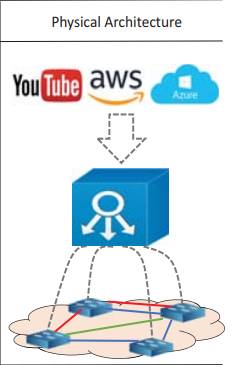
\includegraphics[height=6cm]{../image/arch phy}
	\end{center}
	\caption{Architecture-physique}
\end{figure} 

\section{Les fonctionnalités du Cisco Viptela SD-WAN }

Le Cisco Viptela SD-WAN offre  plusieurs fonctionnalités pour répondre aux besoins de connectivité réseau .
\subsection{Gestion centralisée  }

A travers vManage,on peut assurer l’administration centralisé du système, vManage représente le point principal de surveillance, d'inspection et de configuration de l'infrastructure du réseau. Des options diverses, comme montre la figure , sont mises à disposition grâce à elle.
\begin{figure} [H]
	\begin{center}
		\centering
		\hspace*{-0.5cm}
		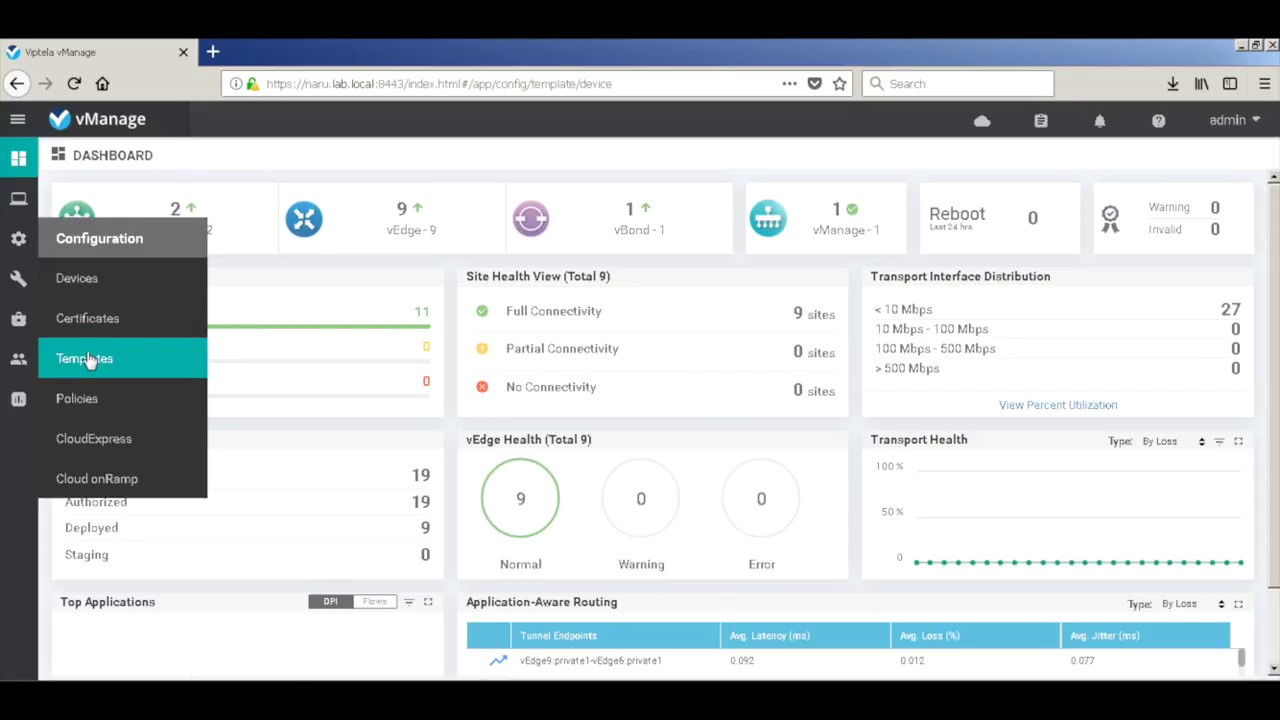
\includegraphics[height=7cm,width=10cm]{../image/Vmanage}
	\end{center}
	\caption{Interface vManage}
\end{figure} 
\subsubsection{Zero-touch provisioning (ZTP)   }
\begin{itemize}
	\item[$\bullet$]\textbf{  Principe :} 
	
	ZTP permet de configurer automatiquement de nouveaux équipements réseau sans intervention manuelle sur le périphérique lui-même, ce qui  simplifie et accélère le processus de déploiement.
\end{itemize}
\begin{itemize}
	\item[$\bullet$]\textbf{Mécanisme :} 
	
	Au début, le vEdge ou le cEdge reçoit l'adresse IP de l'ISP (Internet Service Provider). Dès qu'il est connecté au fournisseur de services, cela est réalisé grâce à DHCP (Dynamic Host Configuration Protocol), qui est configuré du côté du fournisseur de services. Par la suite, le Edge possède une URL ZTP prédéfinie et il peut maintenant atteindre le serveur DNS Viptela. En utilisant l'URL ZTP, le vEdge établit une connexion avec le serveur ZTP, où il vérifie son numéro de série, puis il est redirigé vers l'orchestrateur vBond qui vérifie lui-même le numéro de série et le certificat. Une connexion sécurisée est donc établie entre le Edge et vBond, formant ainsi le plan de contrôle du réseau. Une fois l'authentification du Edge effectuée, vBond envoie l'adresse IP de vManage et vSmart à l'Edge, et informe les autres contrôleurs de ce nouveau périphérique. Après avoir assuré son authenticité, vManage envoie une configuration prédéfinie vers le Edge, qui reçoit aussi la politique par vSmart. De cette façon, le Edge est correctement intégré au SD-WAN overlay et est prêt à échanger des messages OMP.
	
\begin{figure} [H]
	\begin{center}
		\centering
		\hspace*{-0.5cm}
		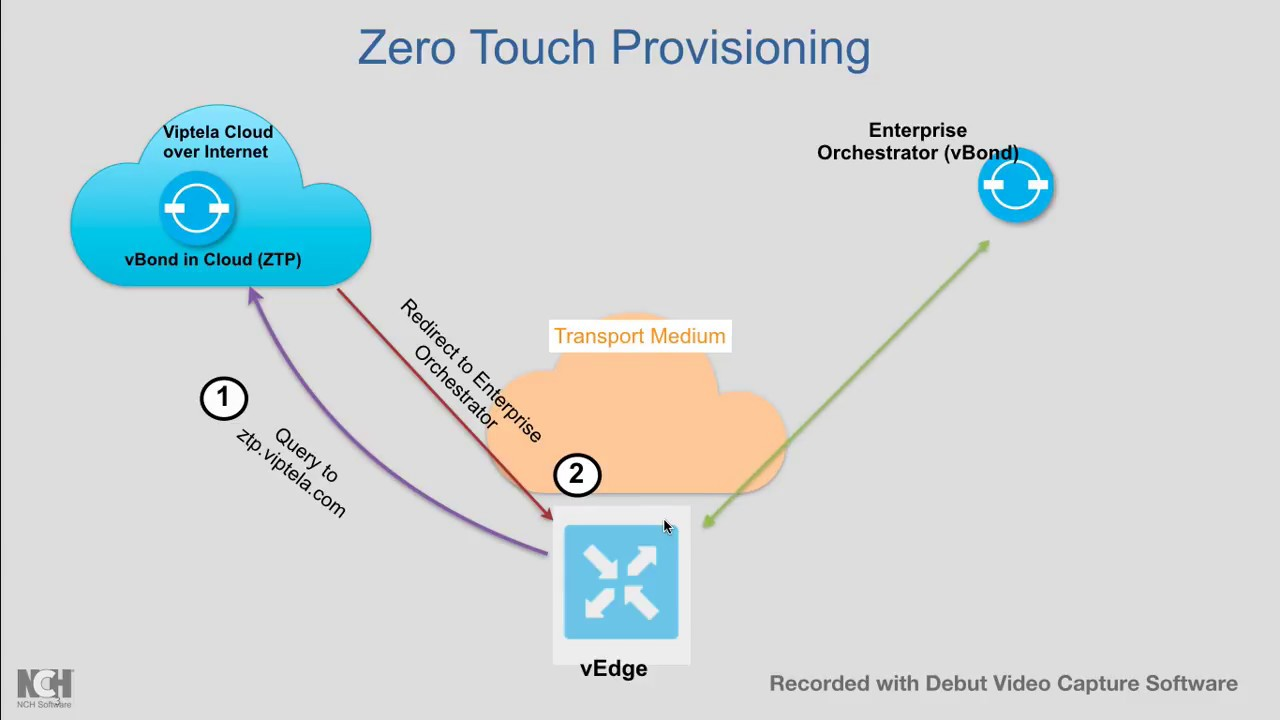
\includegraphics[height=7cm,width=10cm]{image/zttp}
	\end{center}
	\caption{Zero Touch Provisioning}
\end{figure} 
\end{itemize}
\subsubsection{Visibilité des applications  }

La visibilité des applications dans SD-WAN permet au client de voir à travers toute l'infrastructure jusqu'au niveau des flux des applications spécifiques.le client peut observer et comprendre le trafic réseau généré par différentes applications utilisées dans son environnement. 

Cette visibilité offre plusieurs avantages dans  l’identification rapide  de la source du problème, en examinant les flux d'application correspondants.

\subsubsection{Gestion des alertes et des notifications   }

les administrateurs peuvent obtenir des rapports de problème de bout en bout sans traçage.

Lorsqu'un problème critique est détecté  ou une situations qui nécessite  une intervention immédiate, sdwan génère automatiquement des alertes ou des notifications pour que les administrateurs peuvent être informés en temps réel.

\subsubsection{Rapidité d’exécution et Fiabilité Renforcée  }
Dans les réseaux traditionnels,la configuration est assurer via le cli , on se connecte au peripherique via TELNET/SSH ou CONSOLE et on peut modifier la configuration par la suite mais cela nécessite beaucoup de temps pour apporter des modifications massives à la configuration de plusieurs appareils.c’est pour cela il est bien évidement nécessaire d’avoir une autre solution, on parle ici de l'approche centralisée recommandée pour configurer les appareils, cest la configuration Via l'interface graphique vManage, elle est plus fiable en offrant un minimum d’erreurs dans la configuration, peut facilement évoluer et prend en charge l'automatisation, les sauvegardes et la récupération.
Le processus de configuration des nœuds SD-WAN de Cisco via l'interface graphique vManage s'effectue en appliquant des device templates à un ou plusieurs appareils. Une template  contient l'ensemble de la configuration d'un appareil. Lorsque vManage fournit la configuration d'un nœud, il agit comme une source unique de vérité et "verrouille" l'appareil dans un mode de configuration appelé "vManage mode". Cela signifie que les changements de configuration ne peuvent être appliqués que via vManage et que les changements via CLI ne sont pas autorisés.   
Lorsque vManage fournit  la configuration d'un périphérique, il devient la source de référence unique et le périphérique est verrouillé dans un mode de configuration appelé "mode vManage". C’est-à-dire  que seules les modifications de configuration effectuées via vManage sont autorisées, et que les modifications via (CLI) ne sont pas autorisés.

Une template peut être basé sur des features ou CLI , Les templates basées sur  les features peuvent être réutilisés sur plusieurs périphériques . Cela nous donne une plus grande flexibilité et une plus grande évolutivité.De plus,elles sont plus granulaires que les templates basés sur la CLI, par exemple nous pouvons  modifier qu'une seule fonction spécifique de l'appareil, telle que AAA ou BGP.
\subsection{Flexibilité du transport  }

la flexibilité du transport dans la technologie sdwan se manifeste dans son indépendance du type de connexion utilisée pour acheminer le trafic sur le réseau, comme montre la figure   , tel que MPLS, Internet, ou des liaisons privées dédiées.cela permet aux entreprises de choisir multiples fournisseurs de services, de technologies hybrides (par exemple: combinaison de MPLS et d'Internet), ou même l'utilisation de réseaux sans fil comme le LTE ou la 5G, en fonction de leurs besoins spécifiques, de la disponibilité , la performance, la fiabilité, les exigences de bande passante et les coûts.
\begin{figure} [H]
	\begin{center}
		\centering
		\hspace*{-0.5cm}
		\includegraphics{../image/flexibilité de transport}
	\end{center}
	\caption{Flexibilité de transport}
\end{figure} 
\subsection{Intelligence du routage   }

Les protocoles de routage traditionnels sont basés sur des tables de routage .C’est à dire  que chaque paquet est acheminé saut par saut sur le réseau en fonction de la table de routage de chaque routeur individuel le long du chemin vers la destination. Ce comportement de routage hop-by-hop présente de nombreuses inefficacités  puisqu'il nécessite une configuration manuelle sur plusieurs appareils pour assurer Le chaînage des services .
Pour résoudre la plupart de ces inefficacités, l'architecture SD-WAN de Cisco est divisée en deux parties le réseau sous-jacent underlay et le réseau superposé overlay.La couche inférieure constitue la base de notre SD-WAN. C'est ce qui garantit la communication entre les sites sur le réseau étendu,alors que  c'est l'overlay qui rend le SD-WAN si puissant 



\subsubsection{Réseau Overlay }

Le réseau Overlay est constitué de tunnels IPsec et GRE , formant le tissu overlay, qui se déplacent d'un site à l'autre en utilisant le réseau underlay,afin de fournir la segmentation ,la sécurité et la flexibilité dans le reseau.
Le routage dans le reseau overlay est régi par le protocole OMP (Overlay Management Protocol) , un protocole très similaire à BGP. Le protocole OMP fonctionne sur des connexions DTLS ou TLS sécurisées entre les Edges du WAN et vSmart. le contrôleur vSmart agit comme un réflecteur de route BGP, il reçoit, modifie et ré-annonce les routes des routeurs Edge, mais ne participe jamais au plan de données (dans la transmission des paquets) comme montre la figure.
\begin{figure} [H]
	\begin{center}
		\centering
		\hspace*{-0.5cm}
		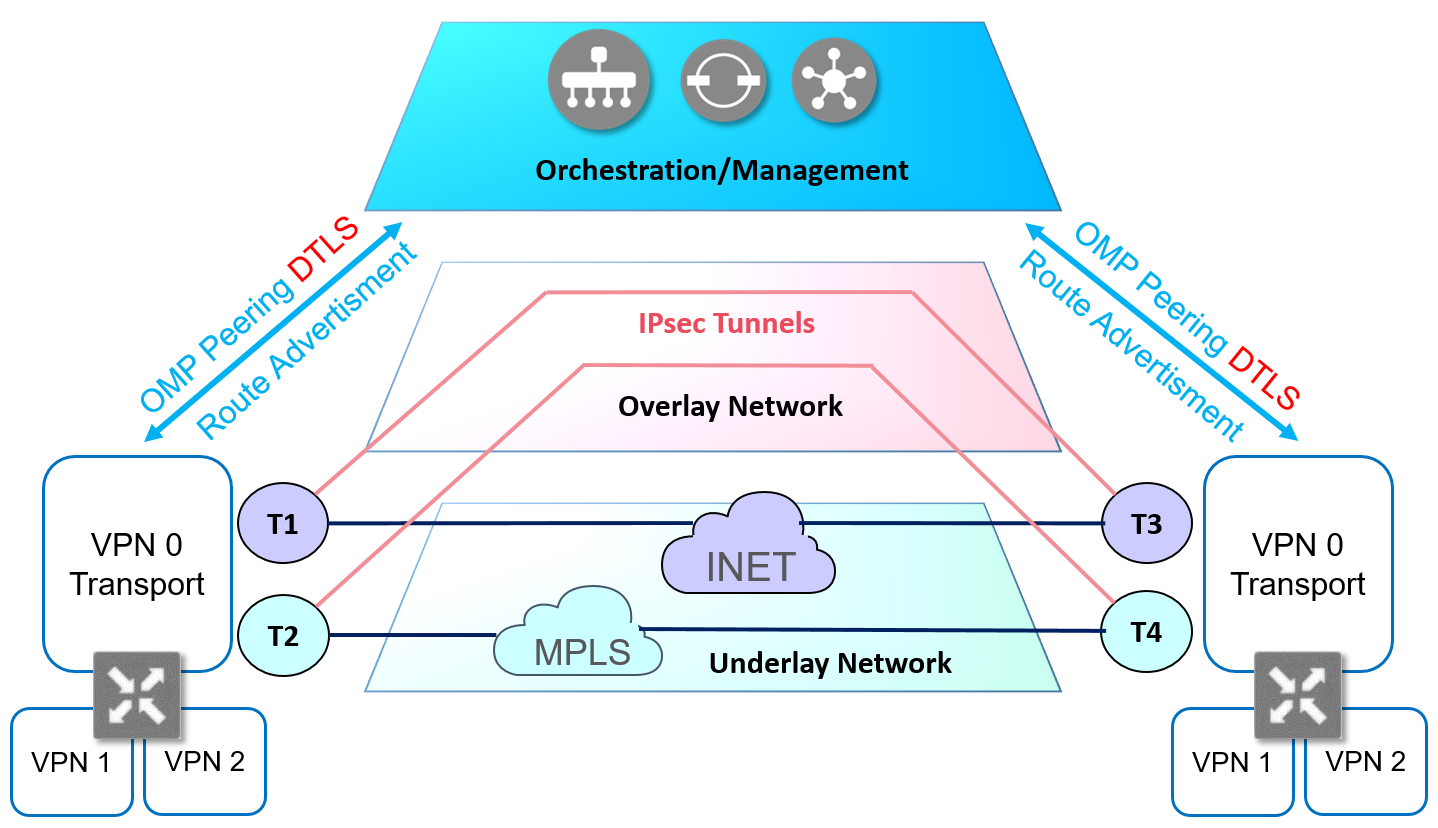
\includegraphics[height=7cm,width=10cm]{../image/Overlay}
	\end{center}
	\caption{Réseau Overlay}
\end{figure} 

Il existe trois types de routes annoncées par OMP :

\begin{itemize}
	\item[$\bullet$]\textbf{  Les routes OMP :} 
	
	Les routes OMP sont utilisées pour l’apprentissage des informations préfixes,ces types de routes peuvent être annoncés dans l'OMP à partir de diverses sources telles que des interfaces connectées, des routes statiques et des protocoles de routage dynamiques tels que OSPF, EIGRP et BGP. Une fois apprises, ces informations de routage sont redistribuées dans le protocole OMP et annoncées au contrôleur vSmart dans la mise à jour OMP.
	Une route OMP Contient les informations suivantes:
	\begin{itemize}
		\item{ Préfixe de destination} 
	\end{itemize}
	\begin{itemize}
		\item{ Préfixe de destination} 
	\end{itemize}
	\begin{itemize}
		\item{ TLOC(Transport Location Identifier):	C’est le prochain saut de la route OMP. Dans le TLOC, il y a trois éléments :
			\begin{itemize}
				\item{ L'adresse IP du système.} 
			\end{itemize}
			\begin{itemize}
				\item{ La couleur: utilisée pour identifier le mode de transport (MPLS ou Internet).} 
			\end{itemize}
			\begin{itemize}
				\item{Le protocole d'encapsulation: peut être GRE ou IPSEC.} 
			\end{itemize}
			\begin{itemize}
				\item{Attributs du préfixe : les attributs tels que l'origine, l'ID de site, le tag, la préférence de chemin et le créateur de la route et l'ID du VPN} 
			\end{itemize}
			
			
\end{itemize}
		
		\newpage
		une route OMP ne sera installée dans la table de transfert du Edge que  si le TLOC next-hop est connu et qu'il existe une session BFD en état actif associée à ce TLOC . La disponibilité des sessions BFD est vérifiée grâce au protocole BFD(Bidirectional Forwarding Detection) qui est un protocole de détection de panne utilisé dans les réseaux informatiques pour détecter rapidement les défaillances de liaison bidirectionnelle entre deux péripheriques de réseau.
	\end{itemize}


	\begin{itemize}
		\item[$\bullet$]\textbf{ Les routes TLOC: } 
	
	
		Une route TLOC (Transport Locator) représente une liaison WAN qui agit comme un point d'extrémité de tunnel dans un environnement SD-WAN. Elle est identifiée de manière unique par trois éléments :
		\begin{itemize}
			\item{ 	Adresse IP système} 
		\end{itemize}
		\begin{itemize}
			\item{ Couleur} 
		\end{itemize}
		\begin{itemize}
			\item{Type d'encapsulation} 
		\end{itemize}
		
		On utilise l'adresse IP système à la place de l'adresse IP de l'interface pour identifier une route TLOC car l'adre sse IP de l'interface peut changer à tout moment, contrairement à l'adresse IP système qui est fixe. Cette stabilité est essentielle car les routes OMP utilisent le next-hop pour pointer vers un TLOC spécifique.De plus ,si un Edge possède plusieurs interfaces de transport connectées à différents fournisseurs WAN, une route TLOC est créée et annoncée pour chaque interface WAN.
		Une route TLOC annonce les attributs d'une terminaison de tunnel SD-WAN, incluant l'encapsulation, la préférence qui est appelée préférence TLOC pour éviter la confusion avec la préférence OMP , l'adresse IP (publique ou privée selon la présence de NAT) et son poids pour la distribution du trafic .
		
	\end{itemize}
	
	\begin{itemize}
		\item[$\bullet$]\textbf{ Les routes de service : } 
		
		Une route de service présente un service réseau, tel qu'un pare-feu ou un équilibreur de charge, connecté à un Edge. Ces services sont souvent déployés dans des endroits centralisés. Le réseau doit être capable de rediriger le trafic depuis n'importe quel site distant à travers ces services, puis de l’acheminer à sa destination initiale.
		La route de service contient les attributs suivants :
		\begin{itemize}
			\item{ ID du VPN  : Le VPN auquel ce service s'applique} 
		\end{itemize}
		\begin{itemize}
			\item{  ID du service: L'identifiant du service définit le type de service annoncé.} 
		\end{itemize}
		\begin{itemize}
			\item{	ID de l'expéditeur : L'adresse IP du Edge qui est à l'origine de la route de service .} 
		\end{itemize}
		\begin{itemize}
			\item{		TLOC : Le TLOC où le service est situé. } 
		\end{itemize}
		
		
	\end{itemize}
	\subsubsection{Réseau Underlay }
	
	Le réseau underlay est l'infrastructure matérielle qui assure la connectivité entre les TLOCs. Sa principale fonction est de permettre le routage selon le next hop, défini par une adresse IP, en utilisant des protocoles de routage traditionnels tels que OSPF, BGP et le routage statique.
	
\subsection{Sécurité}

Les menaces informatiques évoluent et les entreprises ont besoin de solutions de réseau qui offrent une sécurité renforcée. SD-WAN répondent à ce besoin en proposant plusieurs points forts en matière de sécurité.

\subsubsection{Les certificats }
Le SD-WAN s'appuie sur un principe de sécurité qui ne fairt jamais confiance par défaut. C’est à dire chaque Edge qui souhaite participer au réseau doit d'abord s'authentifier et prouver son identité avant d'être autorisé à communiquer.Pour s'authentifier, les Edges utilisent des certificats numériques qui contiennent des informations qui permettent de vérifier l'identité du Edge et de garantir son intégrité.

\subsubsection{Les pare-feu }


Le pare-feu est l'une des formes les plus essentielles de la sécurité des réseaux sur laquelle les organisations s'appuient. 
Cisco a adopté une approche plus moderne en matière de sécurité et a intégré un pare-feu d'entreprise adapté aux applications directement dans les routeurs, éliminant aussi l'extension inutile du réseau sur les sites distants.Prenons l’exemple du Pare-feu applicatif dynamique de type “stateful” qui est capable d’analyser plus de 1400 applications(SD-WAN (3/3) : les 4 avantages principaux de Cisco SD-WAN). Le pare-feu est représenté sous la forme d'une politique de sécurité localisée .Il permet aux équipes de sécurité d'ajouter et de modifier des règles de pare-feu pour des centaines de sites en même temps grâce aux templates et aux fonctions de vManage.  
La séquence d'étapes suivante décrit le mécanisme de configuration de la politique de pare-feu :


\begin{itemize}
	\item{ Définir les zones :une zone source et une zone destination.} 
\end{itemize}
\begin{itemize}
	\item{ Définir une paire de zones : Il est important de définir les paires de zones en tenant compte du sens du trafic prévu.} 
\end{itemize}
\begin{itemize}
	\item{ Créer une politique de sécurité : elle contient toutes les politiques telles que Firewall, IPS, URLF, AMP, etc.}
	\begin{itemize}
		\item{1.Définir une politique de pare-feu.} 
	\end{itemize}
	\begin{itemize}
		\item{ 2.Définir des règles de trafic .} 
	\end{itemize}
	\begin{itemize}
		\item{3.Appliquer la politique de pare-feu à une paire de zones.} 
	\end{itemize}
	
	
\end{itemize}
\begin{itemize}
	\item{ Attacher la politique de sécurité à une template .} 
\end{itemize}

\subsubsection{Les IPS }

Ils dont des systèmes de prévention des intrusions qui analyse le trafic qui circule dans le réseau, Ils utilisent un ensemble de règles prédéfinies, appelées signatures, pour identifier les comportements malveillants.Prenons l’exemple de SNORT qui analyse le trafic réseau en temps réel, ce qui permet de détecter les intrusions et les attaques dès qu'elles se produisent.SNORT travaille en collaboration avec Talos qui fournit des mises à jour automatiques des signatures, ce qui permet de garantir que le système est toujours à jour et capable de détecter les dernières menaces.

\subsubsection{SaSe }
Secure Access Service Edge (SASE) vise à unifier le réseau et la sécurité en une seule solution
Plutôt que de déployer séparément des pare-feu, des systèmes de prévention des intrusions (IPS), des serveurs DNS sécurisés et d'autres outils de sécurité. Cela nous permet de gérer  plus efficacement les politiques de sécurité,de réduire la complexité de l'infrastructure et améliorer la visibilité et le contrôle du réseau.
Le SaSe comporte trois éléments principaux qui travaillent ensemble pour fournir une solution réseau sécurisée et performante pour les entreprises modernes,comme montre la figure. 
\begin{figure} [H]
	\begin{center}
		\centering
		\hspace*{-0.5cm}
		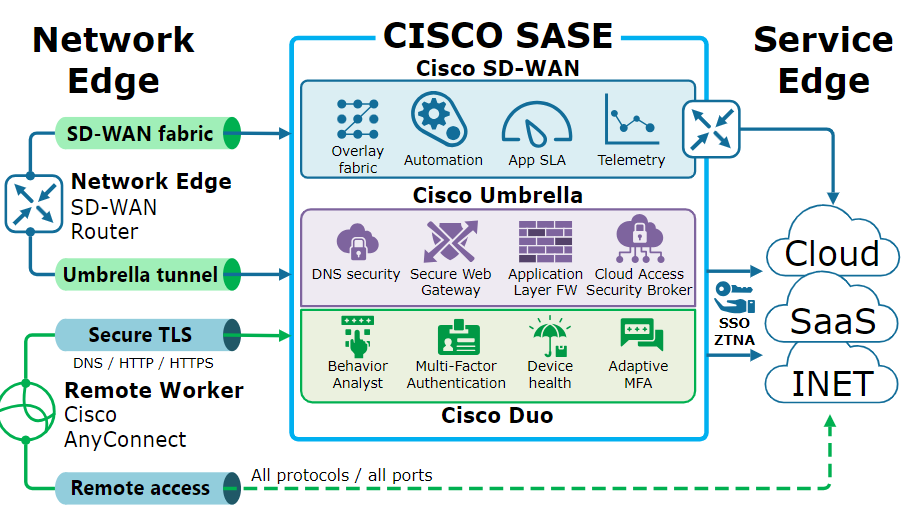
\includegraphics[height=7cm,width=14cm]{../image/sas}
	\end{center}
	\caption{SaSe}
\end{figure} 
\begin{itemize}
	\item[$\bullet$]\textbf{  SD-WAN :} 
	
	Il Gère la connectivité WAN entre les sites et le cloud ,il permet un accès direct à Internet (DIA) dans les sites distants et s'intègre automatiquement avec Umbrella SIG.
\end{itemize}
\begin{itemize}
	\item[$\bullet$]\textbf{ Umbrella SIG(Secure Internet Gateway)  } 
	
	elle fournit une sécurité basée sur le cloud aux utilisateurs distants et remplace les méthodes de sécurité traditionnelles sur site (pare-feu, IPS, proxy).Elle peut aussi combiner plusieurs fonctions de sécurité ,pare-feu cloud, une passerelle web sécurisée (SWG), une inspection de la couche DNS, un courtier de sécurité d'accès en nuage (CASB), une prévention de la perte de données (DLP) et une isolation du navigateur à distance (RBI) en un seul service fourni en nuage qui s'intègre de manière transparente avec le SD-WAN.
\end{itemize}
\begin{itemize}
	\item[$\bullet$]\textbf{ Duo Network Gateway (DNG)} 
	Il fournit un accès sécurisé aux ressources internes pour les utilisateurs distants et élimine la nécessité de gérer les identifiants VPN.De plus il ajoute une couche supplémentaire de sécurité avec l'authentification multifacteur (MFA) et permet un contrôle d'accès granulaire par application et par groupe d'utilisateurs ce qui garantit que seuls les utilisateurs et les appareils autorisés peuvent accéder aux ressources internes.
\end{itemize}
\section{Les Composantes du Cisco Viptela SD-WAN  }

Le SD-WAN de Cisco Viptela s'appuie sur divers éléments, comme illustré dans la figure , qui collaborent pour offrir une solution robuste et solide.
\begin{figure} [H]
	\begin{center}
		\centering
		\hspace*{-0.5cm}
		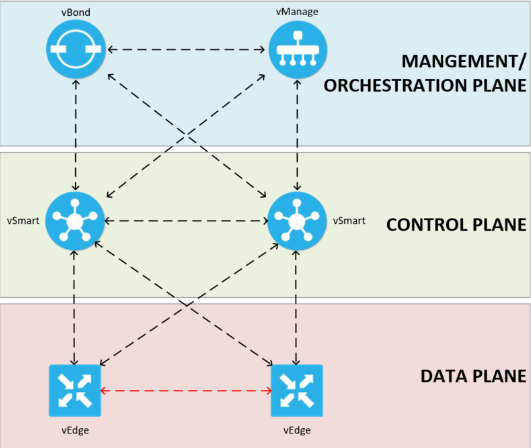
\includegraphics{../image/composantes}
	\end{center}
	\caption{Les Composantes du Cisco Viptela SD-WAN }
\end{figure} 


\subsection{vManage}

vManage est le point de contrôle central dans l'infrastructure SD-WAN. Il offre une interface centralisée pour la configuration, la gestion et la surveillance du réseau. Les administrateurs peuvent établir des politiques de routage, des règles de sécurité, ainsi que diagnostiquer et surveiller les performances du réseau via son tableau de bord.

\subsection{vBond }

vBond agit comme un orchestrateur au sein de l'infrastructure Cisco SD-WAN. Il détermine la construction du réseau et partage ces informations avec les autres composants. C'est le premier point d'accès et d'authentification pour les équipements SD-WAN intégrés à l'overlay (structure logique) , il conserve la liste de tous les équipements autorisés à rejoindre l'overlay SD-WAN. En outre, vBond facilite le Traversal NAT (NAT-T) au sein de l'architecture SD-WAN. La provision sans intervention et la diffusion des données de contrôle et de gestion font  partie des responsabilités assurées par Cisco vBond.

\subsection{vSmart }
vSmart est le composant clé du plan de contrôle dans l'architecture SD-WAN de Cisco. Il est le cerveau des solutions, Il collecte des informations sur l'état du réseau, les politiques de routage et les performances des liaisons. En fonction de ces données, le vSmart prend des décisions de routage intelligentes et distribue les politiques aux autres périphériques du réseau. L'échange d'informations de routage se fait via le contrôleur vSmart et non directement avec les autres sites distants. Vsmart  agit  aussi comme un "route reflector" dans le monde BGP en annonçant ou en filtrant les routes de l’overlay Cisco SD-WAN aux routeurs Edges.
\subsection{Les Edges }

Ils existent plusieurs périphériques dans Cisco SD-WAN Viptela. Ils jouent des rôles spécifiques dans l'architecture du sdwan avec une différence dans leur emplacement de déploiement et leur optimisation pour des environnements particuliers.
\subsubsection{   vEdge  (Virtual Edge) }

Le vEdge est un périphérique de bordure SD-WAN déployé sur site, il peut être  dans un datacenter ou un environnement cloud. Il agit comme un point d'entrée et de sortie pour le trafic en  assurant son acheminement entre les différents sites distants et en  établissant des tunnels sécurisés pour garantir la connectivité avec les autres périphériques vEdge. Il communique avec le vSmart et le vBond pour le contrôle et l'orchestration du réseau, tout en assurant le chiffrement des données pour protéger les communications.

\subsubsection{  cEdge  (Cloud Edge) }


Le cEdge fonctionne de manière similaire au vEdge,il est déployé dans des environnements cloud publics tels que AWS, Azure ou Google Cloud Platform, afin d'assurer une connectivité SD-WAN optimisée au cloud via des tunnels sécurisés.De plus,il est Capable de s'intégrer avec les services cloud natifs pour améliorer les performances et l'efficacité.




\section*{Conclusion }

Dans ce chapitre, nous avons exploré en détail le Cisco Viptela SD-WAN, Nous avons examiné en profondeur son architecture, ses fonctionnalités et ses composants. Dans le prochain chapitre, nous allons voir  la mise en œuvre pratique de la solution, en décrivant les étapes nécessaires pour déployer et configurer le Cisco Viptela SD-WAN dans un environnement réel.

